\documentclass[11pt]{article}
\usepackage[scaled=0.92]{helvet}
\usepackage{geometry}
\geometry{letterpaper,tmargin=1in,bmargin=1in,lmargin=1in,rmargin=1in}
\usepackage[parfill]{parskip} % Activate to begin paragraphs with an empty line rather than an indent %\usepackage{graphicx}
\usepackage{amsmath,amssymb, mathrsfs, dsfont}
\usepackage{tabularx}
\usepackage[font=footnotesize,labelfont=bf]{caption}
\usepackage{graphicx}
\usepackage{xcolor}
%\usepackage[linkbordercolor ={1 1 1} ]{hyperref}
%\usepackage[sf]{titlesec}
\usepackage{natbib}
\usepackage{../../Tianpei_Report}

%\usepackage{appendix}
%\usepackage{algorithm}
%\usepackage{algorithmic}

%\renewcommand{\algorithmicrequire}{\textbf{Input:}}
%\renewcommand{\algorithmicensure}{\textbf{Output:}}



\begin{document}
\title{Lecture 2: Multi-armed Bandit Problem (MAB)}
\author{ Tianpei Xie}
\date{ Dec 27th., 2017 }
\maketitle
\tableofcontents
\newpage
\section{Multi-armed Bandits}
Compared to supervised learning where the training samples are used to \textbf{instruct} by giving the correct actions, in reinforcement learning, training samples are used to \textbf{evaluate} the actions taken. Purely \emph{\textbf{evaluative feedback}} indicates how good the actions taken was, but not whether or not it was the best or worst action possible, and purely \emph{\textbf{instructive feedback}}, on the other hand, indicates \emph{the correct action to take}, independently of the action actually taken. In their pure forms, these two kinds of feedback are quite distinct: \emph{\underline{evaluative feedback depends entirely on the action taken}}, whereas \emph{\underline{instructive feedback is independent of the action taken}}. In other words, supervised learning enforce each step to be as instructed whereas the reinforcement learning only cares if the end goal is reached, and does not care the process. 

The multi-armed bandit problem is seen as  a reinforcement learning problem with \emph{\textbf{nonassociative}} setting, one that does not involve learning to act in more than one situation (\textbf{only a single state}). 

A\textbf{ \emph{k}-armed bandit problem} is stated as follows:  Consider the following learning problem. You are faced repeatedly with a choice among k different options,
or actions. After each choice you receive a numerical reward chosen from a stationary probability distribution that depends on the action you selected. Your objective is to maximize the expected total reward over some time period, for example, over 1000 action selections, or time steps.

\subsection{Exploration and Exploitation}
Consider a $k$-armed bandit problem, each of the $k$ actions has an expected or mean reward given that action is selected. We refer it as the \emph{value} of that action. Denote action selected at time $t$ as $A_t$, and the corresponding reward is $R_t$. The value then of an arbitrary action $a_t$  denoted $q_{*}(a)$ is the \emph{\textbf{expected reward}} given that $a$ is selected.  
\begin{align*}
q_*(a) &:= \E{}{R_t \,|\, A_t = a}.
\end{align*} The problem is trivial if we know the value of each action: the optimal  solution is to select the action with highest value.  Assume that we do not know the action values with certainty. Denote the estimated value of action $a$ at time step $t$ as $Q_t(a)$. We would like $Q_t(a)$ to be close to $q_*(a)$. 

At any time step, given estimates of values for all actions, we can choose one with highest estimated value. The corresponding action is called \emph{\textbf{greedy action}}, and the strategy we use is referred as \emph{exploiting} your current knowledge of the values of actions. Instead, if an non-greedy action is selected, we can improve the estimate of value for that action. This strategy is called \emph{exploration}. 

Exploitation is the right thing to do to maximize the expected reward on the one step, but exploration may produce the greater total reward in the long run.  Because it is not possible both to explore and to exploit with any single action selection, one often refers to the "tradeoff" between exploration and exploitation.  In theory, many sophisticated methods have been proposed to balance the exploration and exploitation, under strong assumptions that may not holds in practice. %By exploration, the reward may be lower in the short term, but since we improve our estimates, in  long term we can exploit them many times.  

\section{Methods}
\subsection{Action-value Methods}
The natural way to estimate the expected rewards is to average the rewards actually received: 
\begin{align}
Q_t(a) &:= \frac{\sum_{i}^{t-1} R_i \cdot \ind{A_i = a}}{\sum_i^{t-1} \ind{A_i = a}} \label{eqn: action_val_methods}
\end{align} and $Q_t(a) = 0$ if the denominator is zero. By Law of large numbers, $Q_t(a) \rightarrow q_*(a)$ as $t\rightarrow \infty$.  This is the sample-average method for estimating action values because each estimate is an average of the sample of relevant rewards.

The simplest strategy is: \emph{greedy action selection} method
\begin{align}
A_t &:= \argmax_{a}Q_t(a) \label{expr: greedy_action_selection}
\end{align} Greedy action selection always exploits current knowledge to maximize immediate reward; it spends no time at all sampling apparently inferior actions to see if they might really be better.

Another strategy is $\epsilon$-greedy action selection:
\begin{align}
A_t &= \left\{\begin{array}{cc}
 \argmax_{a}Q_t(a)  & \text{w.p. } 1- \epsilon \\ 
 \text{uniform}(\cA) & \text{w.p. } \epsilon
\end{array}\right. \label{expr: eps-greedy_action_selection}
\end{align} where $\cA: =\set{\text{all actions available}}$. The benefit for $\epsilon$-greedy action selection is that, in the limit as the number of steps increases, every action will be sampled an infinite number of times, thus ensuring that all the $Q_t(a)$ converge to $q_*(a)$.

\begin{figure}
\begin{minipage}[t]{1\linewidth}
  \centering
  \centerline{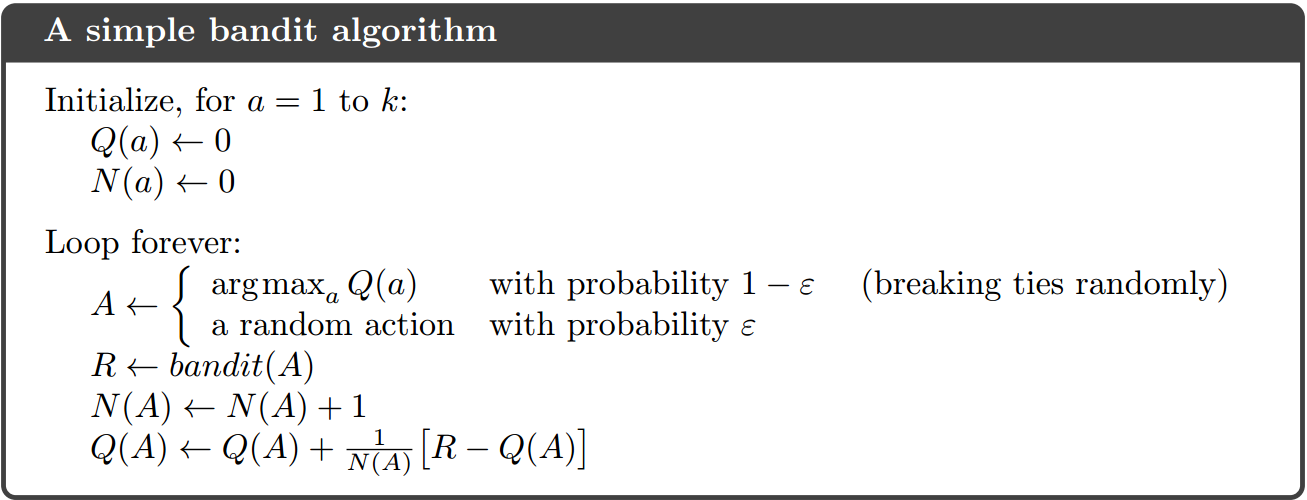
\includegraphics[scale = 0.3]{MAB_epsilon_greedy_algo.png}}
\end{minipage}
\caption{\footnotesize{\textbf{Multi-armed Bandit with $\epsilon$-greedy}.  \citep{sutton2018reinforcement}}}
\label{fig: MAB_epsilon_greedy_algo}
\end{figure}

\subsubsection{Incremental update}
We can compute $\mb{Q}_n:= (Q_n(a): a\in \cA )$ via incremental updates
\begin{align}
\mb{Q}_{n+1} &:= \frac{\sum_i^{n} \mb{R}_{i}}{n} \nonumber\\
&= \frac{1}{n}\paren{\mb{R}_n + (n-1) \mb{Q}_{n}}\nonumber\\
&= \mb{Q}_{n} + \alpha_n(\mb{R}_n - \mb{Q}_n)\;\;\; \text{where }\alpha_n :=\frac{1}{n} \label{eqn: increment_update}\\
\Rightarrow \text{\textbf{new estimate}}&=\text{\textbf{old estimate}} + \text{stepsize}\,\cdot (\text{target} - \text{old estimate})
\end{align} where $\mb{R}_{i}:= (R_{a_{i}}\text{ if }a=a_{i}\text{ otherwise } 0, \text{for all }a\in \cA ).$ Note that $(\mb{R}_n - \mb{Q}_n)$ serves as an \emph{error} term in the estimate. By reducing the error, the estimate is approaching the target, which is presumably a desirable direction in which to move, although it may be noisy. 

\subsubsection{Tracking nonstationary problem}
The averaging method in \eqref{eqn: increment_update} does not fit if the MAB is non-stationary, e,g, if the reward probabilities change over time. In that case, it makes sense to give more weight to recent rewards than to long-past rewards. One of the most popular ways
of doing this is to use a constant step-size parameter $\alpha_n := const \in (0,1]. \;\; $
\begin{align}
\mb{Q}_{n+1} &:= \mb{Q}_{n} + \alpha(\mb{R}_n - \mb{Q}_n)\;\;\nonumber\\
&= \alpha\mb{R}_n + (1-\alpha) \mb{Q}_n\;\;\nonumber\\
&= (1-\alpha)^{n}\mb{Q}_1 + \sum_{i=1}^{n}\alpha(1-\alpha)^{n-i} \mb{R}_i
\end{align} This results in $\mb{Q}_{n+1}$ being a \emph{weighted average} of past rewards and the initial estimate $\mb{Q}_1$. Also see that $(1-\alpha)^{n} + \sum_{i=1}^{n}\alpha(1-\alpha)^{n-i}  = 1$. And the weight depends on $n-i$, i.e. how many rewards ago was observed and it decays \emph{exponentially} as the number of intervening rewards increases. This is also called \emph{exponential recency-weighted average}. 

We can also choose the stepsize $\alpha_n(a)$ as a function of $n$. It assure convergence of equation \eqref{eqn: increment_update} w.p. $1$  if 
\begin{align*}
\sum_{n=1}^{\infty}\alpha_n(a) = \infty \;\; \text{ and }\;\; \sum_{n=1}^{\infty}\alpha^{2}_n(a) < \infty.
\end{align*} The first condition is required to guarantee that the steps are large enough to eventually overcome any initial conditions or random 
fluctuations. The second condition guarantees that eventually the steps become small enough to assure convergence. Note that for $\alpha_n = \frac{1}{n}$, both conditions are satisfied, but for $\alpha_n = \alpha$ const. the second condition is not satisfied, meaning that the process do not converge, which is expected for non-stationary MAB. 

\newpage
\bibliographystyle{plainnat}
\bibliography{reference.bib}
\end{document}